\documentclass{article}

\usepackage{amsmath}
\usepackage{amsthm}
\usepackage{pgfplots}
\pgfplotsset{compat=1.5}

\newtheorem{theorem}{Theorem}

\title{CS325 Project 2 Report}
\author{Erika Crowe and Dean Johnson}

\begin{document}
\maketitle




\subsection*{Correctness of Claim 3}

\begin{theorem}
If $\{z_{1},\ldots,z_{t}\}$ and $\{z'_{1},\ldots,z'_{s}\}$ are two visible sets of lines (each ordered by increasing slope), then the visible subset of $\{z_{1},\ldots,z_{t}\} \cup \{z'_{1},\ldots,z'_{s}\}$ is $\{z_{1},\ldots,z_{i}\} \cup \{z'_{j},\ldots,z'_{s}\}$
\end{theorem}

\begin{proof}Let $\{z_{1},\ldots,z_{t}\} \in Z$. Let $\{z'_{1},\ldots,z'_{s}\} \in Z'$.\newline

\end{proof}

\subsection*{Run-time Analysis}


\begin{tabbing}
  {\sc Algorithm 4: Divide and Conquer}\\
  \qquad \= $n = $number of lines \\
  \> $j = 0$ \\
  \> $i = j+1$\\
  \> $k = i+1$\\
  \> lines$(i,j,k)$ visible = true\\
  \> for $k < n$\\
  \> \qquad \= $y_{jk}$ = y-intersect(lines$(j,k)$)\\
  \> \qquad \= $y_{i}$ = [slope(line$(i)$) $*$ (y-0-intersect(line$(j)$) - y-0-intersect(line$(k)$))]\\
  \> \qquad \= \qquad \= $+$  [y-intersect(line$(i),0$) $*$ slope(line$(k) -$ slope(line$(j)$)]\\ 
  \> \qquad \= if $y_{jk} > y_{i}$\\
  \> \qquad \= \qquad \= line$(i)$ visible = false\\
  \> \qquad \= $j = j+1$\\
  \> \qquad \= $i = i+1$\\
  \> \qquad \= $k = k+1$\\
  \> return
\end{tabbing}

\subsection*{Experimental Correctness}

\emph{Solutions to the instances in the file provided have been submitted to TEACH.}

\subsection*{Experimental Analysis}

% Normal Plot
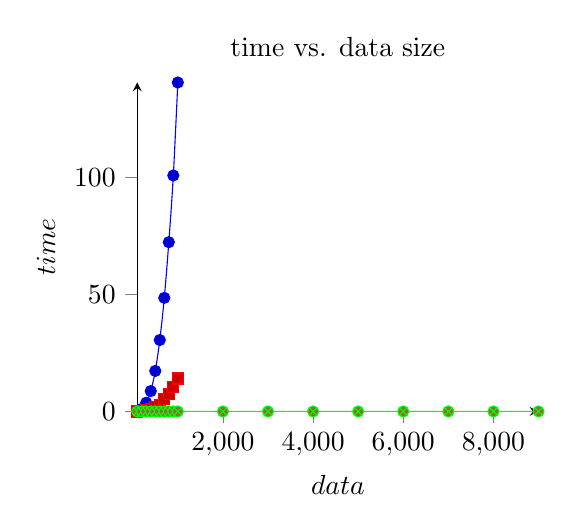
\begin{tikzpicture}
	\begin{axis}[
	title=time vs. data size,
	xlabel={$data$},
	ylabel={$time$},
	width=190pt,
	axis x line=bottom, 
	axis y line=left, 
	tick align=outside
	]
	

		\addplot+[blue,smooth] coordinates {(100,.142428) (200,1.111479) (300,3.739659) (400,8.711271) (500,17.344892) (600,30.563857) (700,48.599125) (800,72.402356) (900,100.940954) (1000,140.711023)};
		\addplot+[red,smooth] coordinates {(100,.020684) (200,.132277) (300,.387687) (400,.965603) (500,1.85595) (600,2.94132) (700,5.17444) (800,7.366091) (900,10.369579) (1000,14.111496)};
		\addplot+[green,smooth] coordinates {(100,.000399) (200,.000399) (300,.000529999999999) (400,.000685000000001) (500,.000826000000004) (600,.000957) (700,.00106699999999) (800,.00123300000001) (900,.00135700000004) (1000,.00151199999999) (2000,.00335699999999) (3000,.00521499999996) (4000,.00500099999999) (5000,.00730500000003) (6000,.0122679999999) (7000,.013183) (8000,.011028) (9000,.013519)};
	\end{axis}
\end{tikzpicture} %


\hskip 10pt %

% Log Log Plot
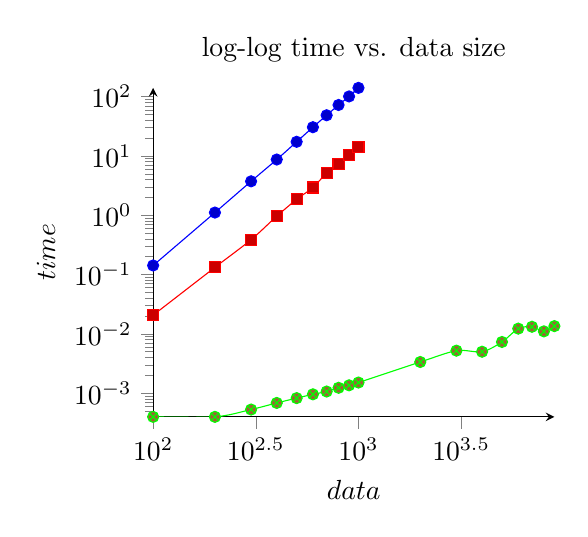
\begin{tikzpicture}
	\begin{loglogaxis}[
	title= log-log time vs. data size,
	xlabel={$data$},
	ylabel={$time$},
	width=190pt,
	axis x line=bottom, 
	axis y line=left, 
	tick align=outside,
	]
		\addplot+[blue,smooth] coordinates {(100,.142428) (200,1.111479) (300,3.739659) (400,8.711271) (500,17.344892) (600,30.563857) (700,48.599125) (800,72.402356) (900,100.940954) (1000,140.711023)};
		\addplot+[red, smooth] coordinates {(100,.020684) (200,.132277) (300,.387687) (400,.965603) (500,1.85595) (600,2.94132) (700,5.17444) (800,7.366091) (900,10.369579) (1000,14.111496)};
		\addplot+[green, smooth] coordinates {(100,.000399) (200,.000399) (300,.000529999999999) (400,.000685000000001) (500,.000826000000004) (600,.000957) (700,.00106699999999) (800,.00123300000001) (900,.00135700000004) (1000,.00151199999999) (2000,.00335699999999) (3000,.00521499999996) (4000,.00500099999999) (5000,.00730500000003) (6000,.0122679999999) (7000,.013183) (8000,.011028) (9000,.013519)};
	\end{loglogaxis}
\end{tikzpicture} %

\subsection*{Extrapolation and Interpolation}

\begin{enumerate}
\item \emph{The biggest instances that could be solved within one hour were not able to be determined.}
\item \begin{enumerate}
\item Algorithm 1 (blue) slope is $\frac{\log(48.599125/8.711271)}{\log(700/400)} = 3.072$
\item Algorithm 2 (red) slope is $\frac{\log(5.17444/.965603}{700/400} = 2.99$
\item Algorithm 3 (green) slope is $\frac{\log(.00106699999999/.000685000000001}{700/400} = .792$
\end{enumerate}
It appears that Algorithms 1 and 2 are similar enough to each other to be $\theta$ to each other, but Algorithm 3 increases at such a lower rate that it is closer to $O$ for both 1 and 2.
\end{enumerate}

\end{document}
